\documentclass[brazil]{beamer}
\usepackage{beamerthemesplit}
\usepackage[brazilian]{babel}
\usepackage[utf8]{inputenc}
\usepackage{color}
\usepackage{xcolor}
\usepackage{graphicx}
%\usepackage{subcaption}
\usepackage{float}
\usepackage{wrapfig}
\usepackage{amssymb}
\usepackage{amsmath}
\usepackage{fancybox}
\usepackage{ulem}
\usepackage{listings}
\usepackage{upquote}
\usetheme{JuanLesPins}
%\usetheme{Warsaw}
%\usetheme{CambridgeUS}
%\usetheme{Malmoe}


%\newcommand{\lyxline}[1][1pt]{%
%  \par\noindent%
%  \rule[.5ex]{\linewidth}{#1}\par}


\title{
  Etherclan
}
\subtitle{
  Rede distribuída descentralizada para localização de outros usuários
}
\author{Henrique Gemignani Passos Lima}

\begin{document}

% ---------------------------------------------------------------------------- %
% Opções de listing usados para o código fonte
% Ref: http://en.wikibooks.org/wiki/LaTeX/Packages/Listings
\lstdefinelanguage{lua}
  {morekeywords={and,break,do,else,elseif,end,false,for,function,if,in,local,
     nil,not,or,repeat,return,then,true,until,while},
   morekeywords={[2]arg,assert,collectgarbage,dofile,error,_G,getfenv,
     getmetatable,ipairs,load,loadfile,loadstring,next,pairs,pcall,print,
     rawequal,rawget,rawset,select,setfenv,setmetatable,tonumber,tostring,
     type,unpack,_VERSION,xpcall},
   morekeywords={[2]coroutine.create,coroutine.resume,coroutine.running,
     coroutine.status,coroutine.wrap,coroutine.yield},
   morekeywords={[2]module,require,package.cpath,package.load,package.loaded,
     package.loaders,package.loadlib,package.path,package.preload,
     package.seeall},
   morekeywords={[2]string.byte,string.char,string.dump,string.find,
     string.format,string.gmatch,string.gsub,string.len,string.lower,
     string.match,string.rep,string.reverse,string.sub,string.upper},
   morekeywords={[2]table.concat,table.insert,table.maxn,table.remove,
   table.sort},
   morekeywords={[2]math.abs,math.acos,math.asin,math.atan,math.atan2,
     math.ceil,math.cos,math.cosh,math.deg,math.exp,math.floor,math.fmod,
     math.frexp,math.huge,math.ldexp,math.log,math.log10,math.max,math.min,
     math.modf,math.pi,math.pow,math.rad,math.random,math.randomseed,math.sin,
     math.sinh,math.sqrt,math.tan,math.tanh},
   morekeywords={[2]io.close,io.flush,io.input,io.lines,io.open,io.output,
     io.popen,io.read,io.tmpfile,io.type,io.write,file:close,file:flush,
     file:lines,file:read,file:seek,file:setvbuf,file:write},
   morekeywords={[2]os.clock,os.date,os.difftime,os.execute,os.exit,os.getenv,
     os.remove,os.rename,os.setlocale,os.time,os.tmpname},
   alsodigit = {.},
   sensitive=true,
   morecomment=[l]{--},
   morecomment=[s]{--[[}{]]},
   morestring=[b]",
   morestring=[d]',
   morestring=[s]{[[}{]]},
  }

\frame{
  \titlepage
  Orientador: Prof. Dr. Daniel Macedo Batista
}

\frame{\tableofcontents}

%-------------------------------------
\section{Introdução: Motivações e Objetivos}
%-------------------------------------
\begin{frame}[fragile]
  \frametitle{Motivações}
  Interesse em:
  \begin{itemize}
    \item Jogos eletrônicos.
    \item Redes de computadores.
  \end{itemize}
  \pause
  \vspace{30pt}
  Uma forma comum de juntar os dois é um jogo multijogador através da Internet!
\end{frame}
%-------------------------------------
\begin{frame}[fragile]
  \frametitle{Motivações - Internet}
  Mas quando se fala de um projeto open-source, quais dificuldades surgem?
  \pause
  \vspace{10pt}
  \begin{enumerate}
    \item Grande parte da lógica nos servidores
        \pause
        \begin{itemize} \item Necessidade de manter servidores potentes, caro. \end{itemize}
    \pause
    \vspace{10pt}
    \item Servidores dedicados por parte dos jogadores
        \pause
        \begin{itemize} \item Como encontrar esses servidores de maneira automatizada? \end{itemize}
  \end{enumerate}

\end{frame}
%-------------------------------------
\frame{
  \frametitle{Proposta de TCC}
  \begin{center}
    \huge{Etherclan}
  \end{center}
  \vspace{20pt}
  \begin{itemize}
    \pause
    \item Rede peer-to-peer, isto é, uma rede descentralizada.
    \pause
    \item Função de encontrar outros membros da rede.
    \pause
    \item Pode ser utilizada por mais de um jogo simultaneamente.
    \pause
    \item Capaz de buscar por membros de um jogo específico.
  \end{itemize}
}
%-------------------------------------
\section{Conceitos}
%-------------------------------------
\begin{frame}
  \frametitle{Peer-to-peer X Cliente-Servidor}
  
    \begin{figure}[h]
      \fbox{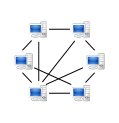
\includegraphics[width=0.45\textwidth]{../poster/p2p-network.png}}
      \fbox{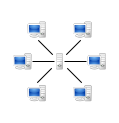
\includegraphics[width=0.45\textwidth]{../poster/server-based-network.png}}
    \end{figure}
  
    Numa rede peer-to-peer cada nó da rede atua como consumidores e
    fornecedores de recursos, em contraste com redes cliente-servidor onde nós
    clientes apenas requisitam serviços de servidores centrais.
  
\end{frame}
%-------------------------------------
\section{Funcionamento da rede}
%-------------------------------------
\begin{frame}
  \begin{center}
    \huge{Funcionamento da rede}
  \end{center}
\end{frame}
%-------------------------------------
\begin{frame}
  \frametitle{Entrando na rede}
  Para entrar na rede, é necessário dois passos.
  \pause
  \begin{enumerate}
    \item Criar um nó.
    \pause
    \item Informar algum membro da rede sobre o novo nó.
  \end{enumerate}
\end{frame}
%-------------------------------------
\begin{frame}
  \frametitle{Bootstrapping}
  
  Mas como eu consigo esse primeiro nó?
  \vspace{20pt}
  \pause
  \begin{itemize}
    \item Lista fixa de IP e porta.
    \pause
    \item Busca cega.
    \pause
    \item Aproveitar alguma outra rede P2P?
  \end{itemize}
\end{frame}
%-------------------------------------
\begin{frame}
  \frametitle{Protocolo de Rede}
  
  Para que dois nós consigam se comunicar, é necessário que ambos sigam um protocolo de rede.
  
  \vspace{20pt}
  \pause
  
  Qual o básico necessário que esse protocolo tem que permitir?
  \begin{itemize}
    \pause
    \item Informar um novo nó na rede.
    \pause
    \item Requisitar uma lista de nós da rede.
  \end{itemize}
\end{frame}
%-------------------------------------
\begin{frame}
  \frametitle{Sobre os Nós}
  
  Antes de se aprofundar no protocolo, quais informações temos sobre cada nó?
  \pause
  \begin{itemize}
    \item Um UUID (Universally Unique IDentifier), segundo RFC 4122.
    \pause
    \item Endereço IP e porta.
    \pause
    \item Lista de serviços fornecidos.
  \end{itemize}
  \vspace{15pt}
  \pause
  Serviços? \\
  \pause
  Funcionam com expansões do protocolo da rede. \\
  Útil para saber se o nó é do mesmo jogo que o seu.
  
\end{frame}
%-------------------------------------
\begin{frame}
  \frametitle{Desenvolvimento do Protocolo}
  
  Estratégia inicial foi listar todas as necessidades do projeto de início,
  similar a como se modela um banco de dados.
  
  \pause
  \vspace{10pt}
  
  \textit{Pessoal:} Pelo menos 1 mês foi gasto travado nesse passo, sem progresso. :( \\
  
  \pause
  \vspace{20pt}
  
  Projeto começou a andar bastante quando a estratégia foi mudada para
  implementar o que precisa para o momento, mudando sempre que necessário,
  seguindo ideologia de programação ágil.
\end{frame}
%-------------------------------------
\section{Resultados}
%-------------------------------------
\begin{frame}
  \begin{center}
    \huge{Resultados}
  \end{center}
\end{frame}
%-------------------------------------
\begin{frame}
  \frametitle{Daemon}
  
  \makebox[\linewidth]{
    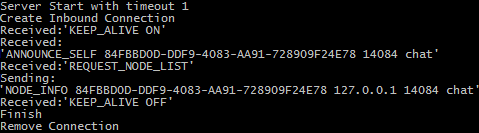
\includegraphics[width=1.2\textwidth]{daemon.png}
  }
  
  \vspace{10pt}
  
  \textbf{Proposta:} fornecer um nó para servir como bootstrap para outros.
  
\end{frame}
%-------------------------------------
\begin{frame}
  \frametitle{Chat}
  
  \begin{figure}
  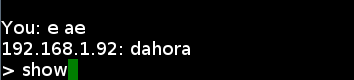
\includegraphics{chat.png}
  \end{figure}
  
  \pause
  
  \textbf{Proposta:} um chat que envia e recebe mensagens para nós da rede, utilizando
  um serviço de nome \textit{chat}. Não possui nomes de usuário, nem confirmação
  de quem recebeu as mensagens enviadas.
  
  \vspace{10pt}
  \pause
 
  Desenvolvido como uma prova de conceito, demonstrou os seguintes pontos:
  \begin{itemize}
    \pause
    \item Funciona!
    \pause
    \item Precisa de melhorias no controle de nós conhecidos
  \end{itemize}
\end{frame}
%-------------------------------------  
\begin{frame}
  \frametitle{Futuro}
  
  \begin{itemize}
    \item Definir estratégias melhores para:
      \begin{itemize}
        \item Considerar um nó como morto
        \item Parar busca por novos nós
        \item Começar outra busca por novos nós
      \end{itemize}
    
    \pause
    \vspace{15pt}
    
    \item Fazer uma biblioteca em C++ para facilitar integração com outros projetos.
      \begin{itemize}
        \item Um projeto em C++ é facilmente exportado para diversas outras linguagens. \tiny{(Ouroboros)}
      \end{itemize}
      
    \pause
    \vspace{15pt}
    
    \item Utilizar em outros projetos!
      
  \end{itemize}
\end{frame}
%-------------------------------------
\begin{frame}
  \frametitle{kthxbye}
  \begin{center}
    \huge{Fim}
    \\
    \vspace{20pt}
    \tiny{Perguntas?}
  \end{center}
\end{frame}
%-------------------------------------
\end{document}

